\hypertarget{chapter6}{}
\chapter{Computer Applications}

Writing computer applications has been an integral process in the creation of the submitted work. The development of computer applications during the period of research has run simultaneously with my aesthetic and musical concerns. From composition and conception to performance and realization, producing computer applications and making music have merged within the same creative process. Consequently, my musical practice has become deeply connected with computer programming and the use of computer applications. It is also worth mentioning that the applications developed as part of the creative process have been specifically devised for my particular musical interests and that the process of their development has influenced my own musical thought up to the point that it has changed the way I think about musical practice and the act of composing. Additionally, these computer applications have had significant effect over varying aspects of the \emph{musical result} and their impact is apparent in the submitted work. Therefore, understanding how these applications work might also give an insight into my musical output. At this point, I would also like to clarify that these applications do not serve a function beyond the idiosyncratic practices that constitute my creative process. In other words, these applications were written only taking in consideration my own artistic and musical concerns and therefore they do not aim at contributing to the scientific and technological developments of computer music. Instead, they only represent a set of tools and documentation that other artists, musicians and composers might find useful in understanding my work and hopefully may also inform their own practice.

In \hyperlink{chapter4}{Chapter 4}, I explained some of the potential that technology has brought to music and how even though technological advancements do not necessarily represent artistic developments, they do provide with new possibilities for artistic innovation. It is because of these possibilities that I have become recently interested in using digital technology to create music. I am also particularly interested in using technology for the strategies of appropriation described in \hyperlink{chapter5}{Chapter 5}... 
 
In this chapter, I will explain in detail a number of key computer applications that were developed together within my musical practice\footnote{The computer code for all of the applications and compositions developed as part of the submitted work can be found at my public code repository at \href{http://github.com/freuben/}{\texttt{http://github.com/freuben/}}.}. These applications were written in the \mbox{SuperCollider}\footnote{James McCartney, SuperCollider, 1996. URL: \href{http://www.audiosynth.com/}{\texttt{http://www.audiosynth.com/}}} programming language. I decided to use SuperCollider as a platform to develop these computer applications because it integrates a powerful audio synthesis server using state-of-the-art technology with the versatility and capabilities of an object-oriented-programming (OOP) language. I chose SuperCollider over other data flow programming applications like \href{http://www.cycling74.com/}{Max/MSP} and \href{http://puredata.info/}{Pure Data} (Pd) because of its robust synthesis server and the advantages of abstraction of a high-level OOP language.\footnote{See \hyperlink{mccartney}{McCartney, (2002)}, pp. 61-68, for a discussion about the differences between SuperCollider and Max/MSP, Pd and Csound.} Another advantage I saw in using SuperCollider is the fact that it is an open source application, which means that the code in which it is written is available for free and can be modified. Most of the computer applications I developed and which will be discussed in this chapter are written as SuperCollider classes,\footnote{SuperCollider classes are descriptions of the structure and implementation of a set of objects that represent the instances of the class.} but some of them are extensions of already existing classes or code that can be evaluated in real-time in the interpreter. The applications discussed in this chapter were used in various of the works submitted and constitute compositional strategies that reflect some aesthetic concerns that are recurrent in my work.

\section{Spectral Tracking}

In \hyperlink{chapter5}{Chapter 5}, I briefly explained how spectralism and C. Barlow: \emph{Synthrumentation} influenced my work.

Fast Fourier Transform (FFT)


Midi

\subsection{Partial Tracking}

Spectrum analysis for dynamics, pitch and rhythm extraction. 

\hypertarget{partrack}{}
\subsubsection{PartialTracker}

\href{http://github.com/freuben/FedeLib/blob/master/PartialTracking/PartialTracker.sc}{PartialTracker} is a SuperCollider class for real-time partial extraction that diminishes the amount of FFT data by selecting the loudest bins and discarding the softer magnitudes with the purpose of having a limited amount of values to be returned as simple arrays for frequency and magnitude. It does so by taking an incoming audio signal, performing an FFT analysis and discarding spectral data in two ways: either by passing only the bins that are above a given magnitude threshold or by selecting a value that returns the strongest number of bins. For this purpose, I used the PV\_MagAbove and PV\_MaxMagN\footnote{PV\_MaxMagN is part of JoshUGens by \href{http://www.realizedsound.net/josh/}{Joshua Parmenter}, which is part of the \href{http://sourceforge.net/projects/sc3-plugins/}{sc3-plugins project}.} phase vocoder unit generators. In order to have access to this data in the language side of SuperCollider, I used PV\_MagBuffer and PV\_FreqBuffer\footnote{PV\_MagBuffer and PV\_FreqBuffer are part of JoshUGens.} to store this information into a buffer. Ones stored in a buffer, the information can be accessed as an array and be manipulated freely. Nevertheless, the buffer stores all of the bins of the FFT and therefore the bins with the magnitudes that were not empty have still to be collected and indexed to access the corresponding frequency values. The resulting arrays therefore only constitute the number of strongest bins, which can be defined by the user. The following code shows an example of the frequency and magnitude arrays for the ten strongest bins:

\begin{verbatim}
[ 128.37791442871, 154.57292175293, 140.25003051758, 246.26268005371, 253.09353637695,
 364.92492675781, 396.52267456055, 1035.068359375, 1037.1043701172, 1241.3063964844 ]; 
 //array of frequencies

[ 1.8754153251648, 4.5471153259277, 5.3137745857239, 2.6146886348724, 1.2295168638229,
  2.5435922145844, 3.215939283371, 2.0944044589996, 2.6014709472656, 2.0559096336365 ]; 
 //array of magnitudes
\end{verbatim}
The purpose of this class is to have easy access to relevant FFT information with the aim to convert frequencies and magnitudes either as Midi messages or as data to be used to control synthesis definitions\footnote{Synthesis definitions, or SynthDefs in SuperCollider represent a description of a set of Unit Generators (UGens) that perform synthesis algorithms in the SuperCollider server.}. The incoming signal can be a live input in a performance situation, or a sound file. Lastly, this class also provides the feature of saving the spectral information trigged by an onset detector with the objective of  creating a Midi file by storing time values and converting the frequency and magnitude data to Midi notes and velocities.

\subsubsection{FFTFilter}

\href{http://github.com/freuben/FedeLib/blob/master/PartialTracking/PartialTracker.sc}{FFTFilter} inherits functionality from \hyperlink{partrack}{PartialTracker} and uses the information of the frequency array to control the bandwidth and center frequency of a two pole resonant filter. This FFT controlled filter is designed to be used to filter a signal with a rich spectral content, such as different types of noise, with the information given by an FFT analysis of another signal that should be more limited in its frequency range. A function is evaluated in a loop in which an argument that can be changed by the user represents the time value between each iteration. This function accesses the highest and lowest frequency values from the array calculated by the PartialTracker functionality every time the loop is evaluated. Since the purpose is to make a smooth line instead of discrete points, the signal must be lagged exponentially to produce a continuous control signal. By following this procedure, it is possible to approximately track the contour of the frequencies that have a stronger presence, given that the settings for the amount of strongest bins and magnitude threshold are appropriate for the specific spectral characteristics of the signal. Figure 4.1 
\begin{figure}[htbp] %  figure placement: here, top, bottom, or page
   \centering
   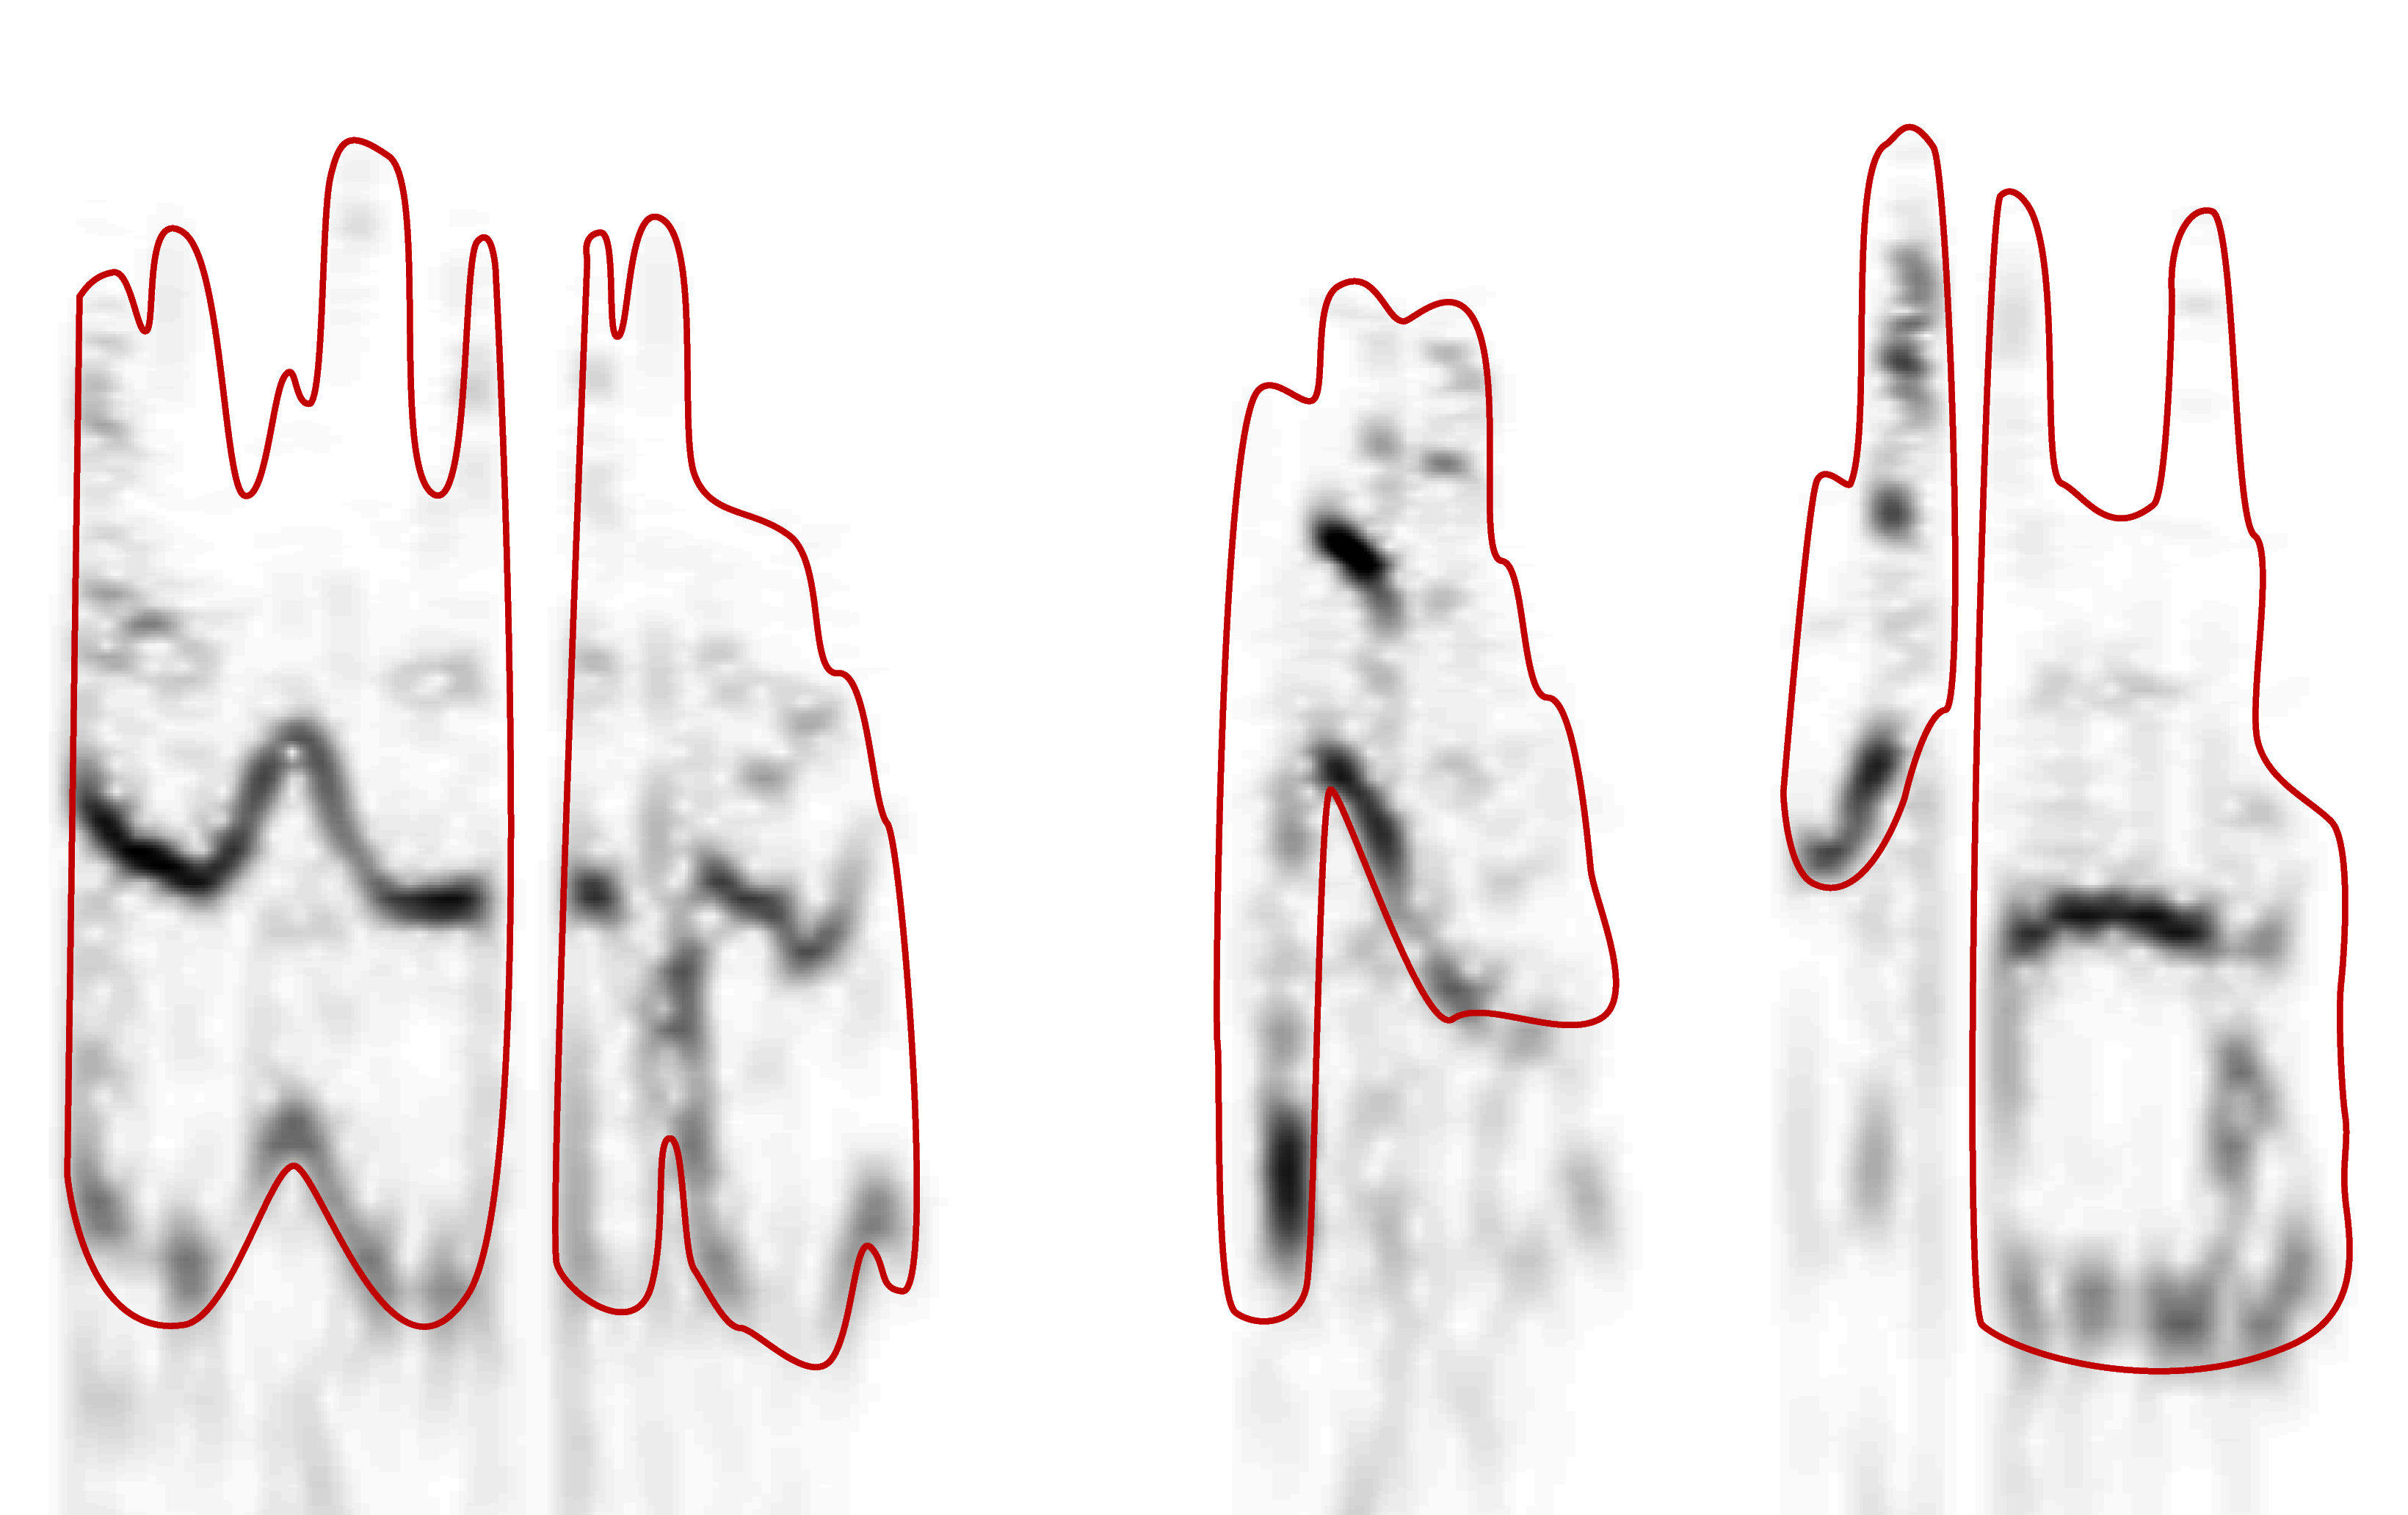
\includegraphics[width=10cm]{Chapter6/spectovocal.tif} %change centimeters for resizeing
   \caption{FFTFilter: Spectral mapping of vocal contour.}
   \label{fig:example}
\end{figure}
shows a spectrogram of speech and how the FFTFilter maps the contour of the vocal signal. Given that the vocal signal has a strong presence in a narrow frequency range, it is ideal to control the filter. FFTFilter therefore uses the continuos signal of the highest and lowest frequencies of the array to calculate the bandwidth and center frequency for the resonant filter. Figure 4.2 shows a visual representation of a fairly noisy signal that has been filtered by the resonant filter following the vocal contour as seen in Figure 4.1. 
\begin{figure}[htbp] %  figure placement: here, top, bottom, or page
   \centering
   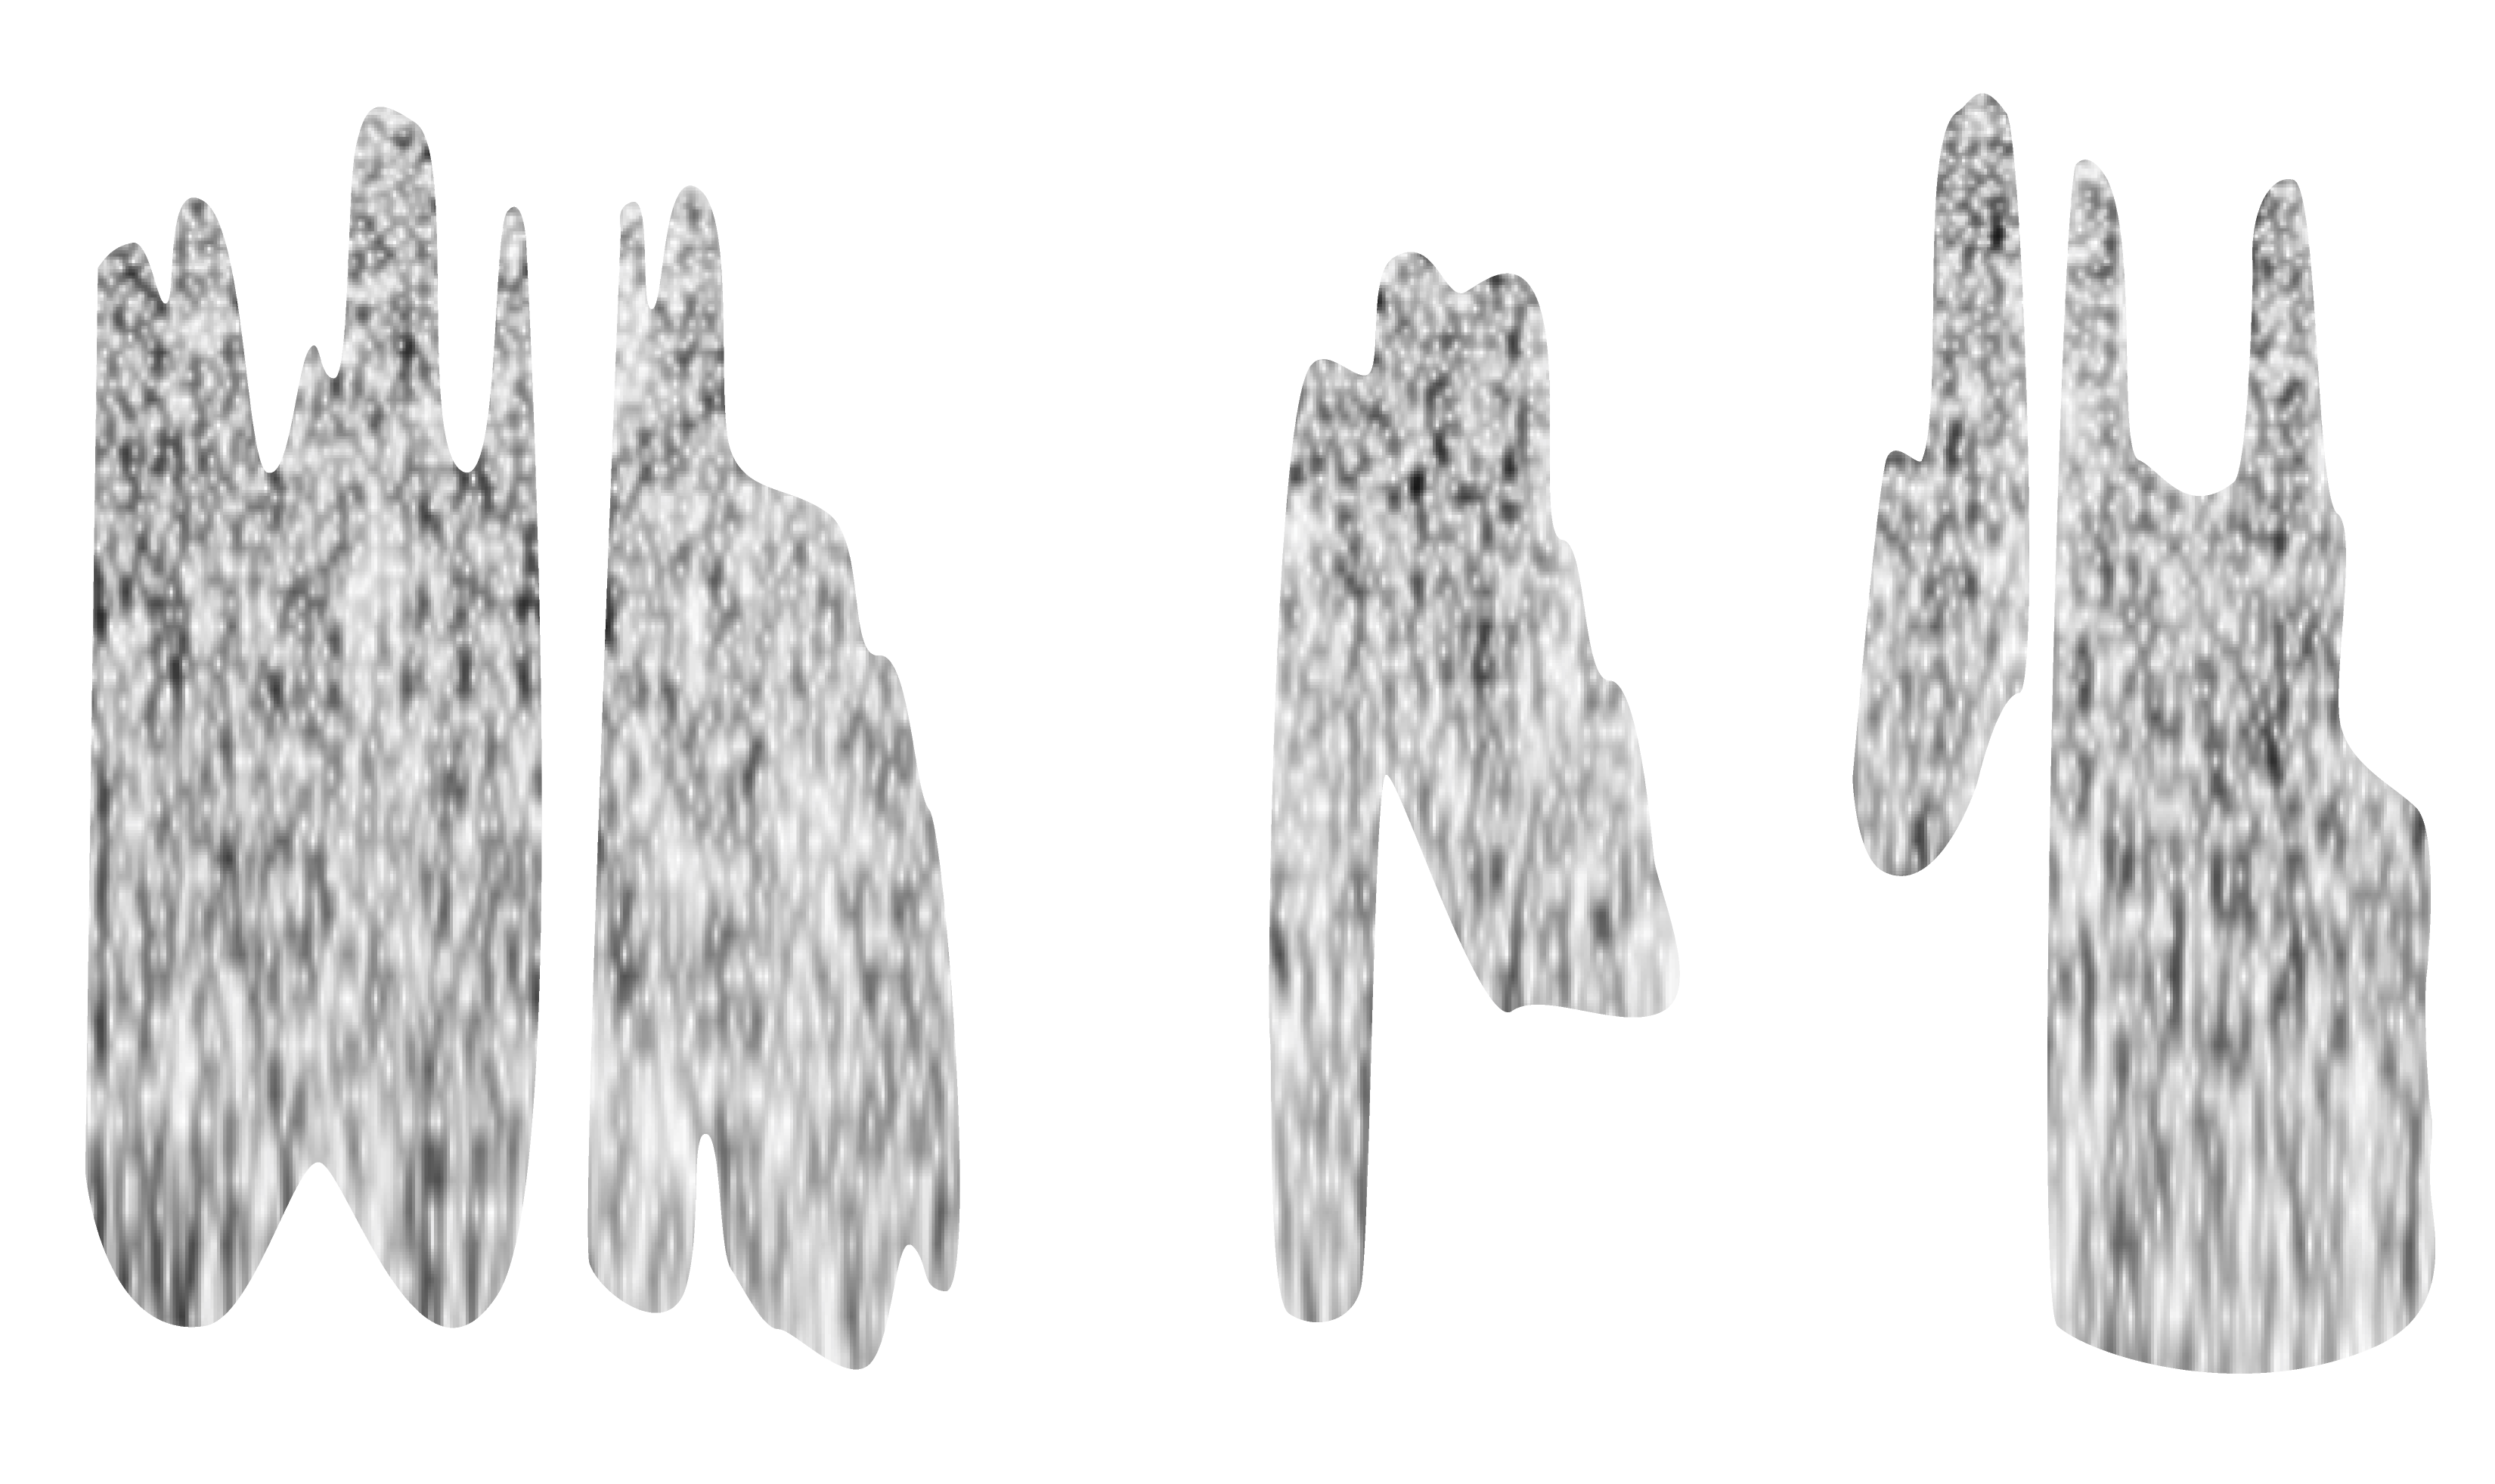
\includegraphics[width=10cm]{Chapter6/spectonoise.tif} %change centimeters for resizeing
   \caption{FFTFilter: Noise filtered by vocal contour.}
   \label{fig:example}
\end{figure}
Ones the trajectory of the filter is set by the frequency data extracted from the FFT, an envelope follower maps the amplitude of the sound that was used as the FFT input to control the amplitude of the resonant filter. By combining the amplitude envelope and frequency contour of one sound to control a resonant filter that is applied to another sound, it is possible to incorporate characteristics of the analyzed sound to the filtered sound source.

\subsection{Spectral Data Extraction and Reduction}

\hypertarget{spearsc}{}
\subsubsection{SpearToSC}

\href{http://github.com/freuben/FedeLib/blob/master/SpearToSC/SpearToSC.sc}{SpearToSC} is a class that takes data from the open source software application called SPEAR\footnote{Klingbeil, Michael (2005), SPEAR, URL: \href{http://www.klingbeil.com/spear/}{http://www.klingbeil.com/spear/}.} and transfers it to an array in SuperCollider. SPEAR uses a variation of the traditional McAulay-Quartieri procedure to represent sounds as individual sine waves (for each partial) with time varying frequency and amplitude.\footnote{See \hyperlink{klingbeil}{Klingbeil (2005)}.} SPEAR provides a graphical representation of a sound\footnote{Spectral analysis, where the y-axis represents frequency in hertz and the x-axis represents time in seconds.} (as seen in Figure 4.3) in which it is possible to select the individual sinusoidal tracks and allows to isolate and access the information for each individual partial. 
\begin{figure}[htbp] %  figure placement: here, top, bottom, or page
   \centering
   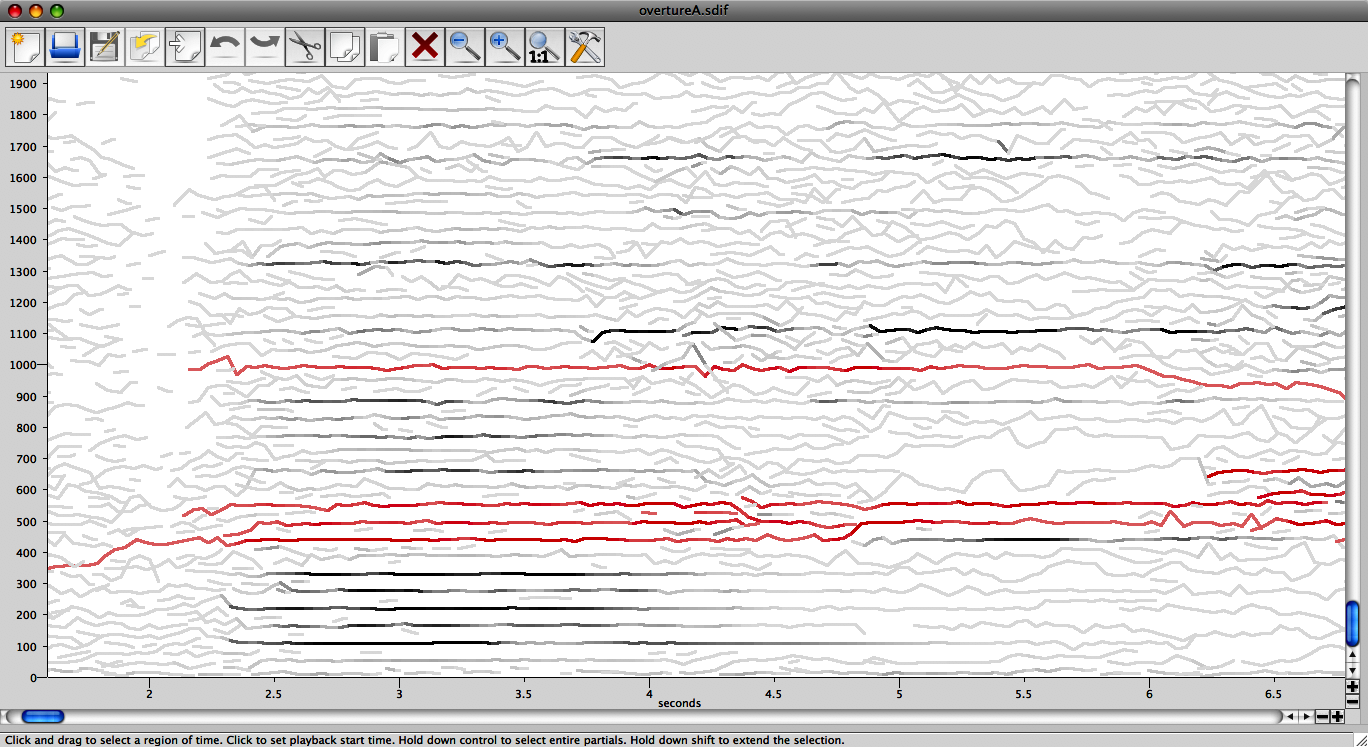
\includegraphics[width=15cm]{Chapter6/Spear1.tif} %change centimeters for resizeing
   \caption{SPEAR graphical interface.}
   \label{fig:example}
\end{figure}
The amplitude and frequency information of each partial is given by frame and can be stored in a text file. SpearToSC reads the text file produced by SPEAR\footnote{SpearToSC reads SPEAR text files in the \emph{Text - Partials} format only.} as a string and strips it into a multidimensional array in SuperCollider. It is therefore possible to access and manipulate this data within the SuperCollider language and server and re-synthesize this information not only with sinusoidal waves, but with any type of unit generator. 

\subsubsection{SpearToMIDI}

\href{http://github.com/freuben/FedeLib/blob/master/SpearToSC/SpearToMIDI.sc}{SpearToMIDI} is a class that inherits functionality from \hyperlink{spearsc}{SpearToSC} and reduces the information given by SPEAR to be used as data to produce a Midi file or to control SuperCollider synthesis definitions. The purpose of this class is to reduce the spectral information to an amount of data that can later produce notated material for a written score, a Midi file or a control system to be used for triggering synthesis algorithms. The data in the text file generated by SPEAR is available by frame and gives too much information for this purpose. Therefore, SpearToMIDI reduces this data in four stages: First, it takes a magnitude threshold argument which gets rid of all of the partial information that lies bellow this value (as seen in Figure 4.4).
\begin{figure}[htbp] %  figure placement: here, top, bottom, or page
   \centering
   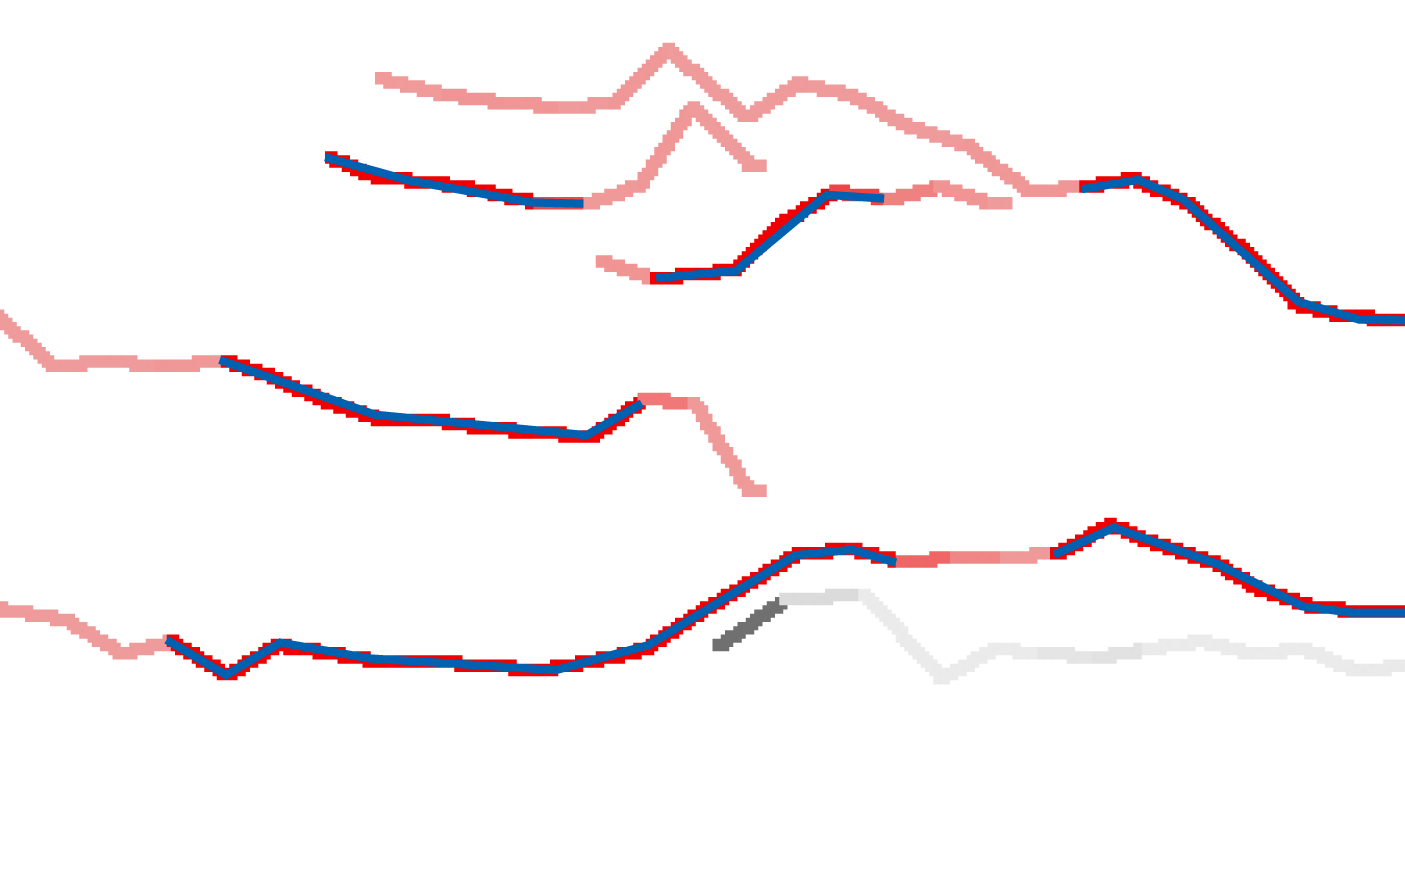
\includegraphics[width=9cm]{Chapter6/Spear2.tif} %change centimeters for resizeing
   \caption{SpearToMIDI: Amplitude threshold selection.}
   \label{fig:example}
\end{figure}\
In other words, it breaks the partial in different groups by introducing silences instead of the data that lies bellow the threshold and at the same time keeps track of the beginning and the end of each group. 

The second stage reduces data with a frequency modulation threshold. Each group is taken as a line and the computer only stores the points in the line which cross a given interval (the modulation threshold). For example, Figure 4.5 shows how the lines representing the groups in Figure 4.4 are traced by selecting the points that cross a given interval.\footnote{The grid represents the intervals as shown in the y-axis. For the purpose of simplification, the diagram doesn't show a logarithmic representation of frequency.} 
\begin{figure}[htbp] %  figure placement: here, top, bottom, or page
   \centering
   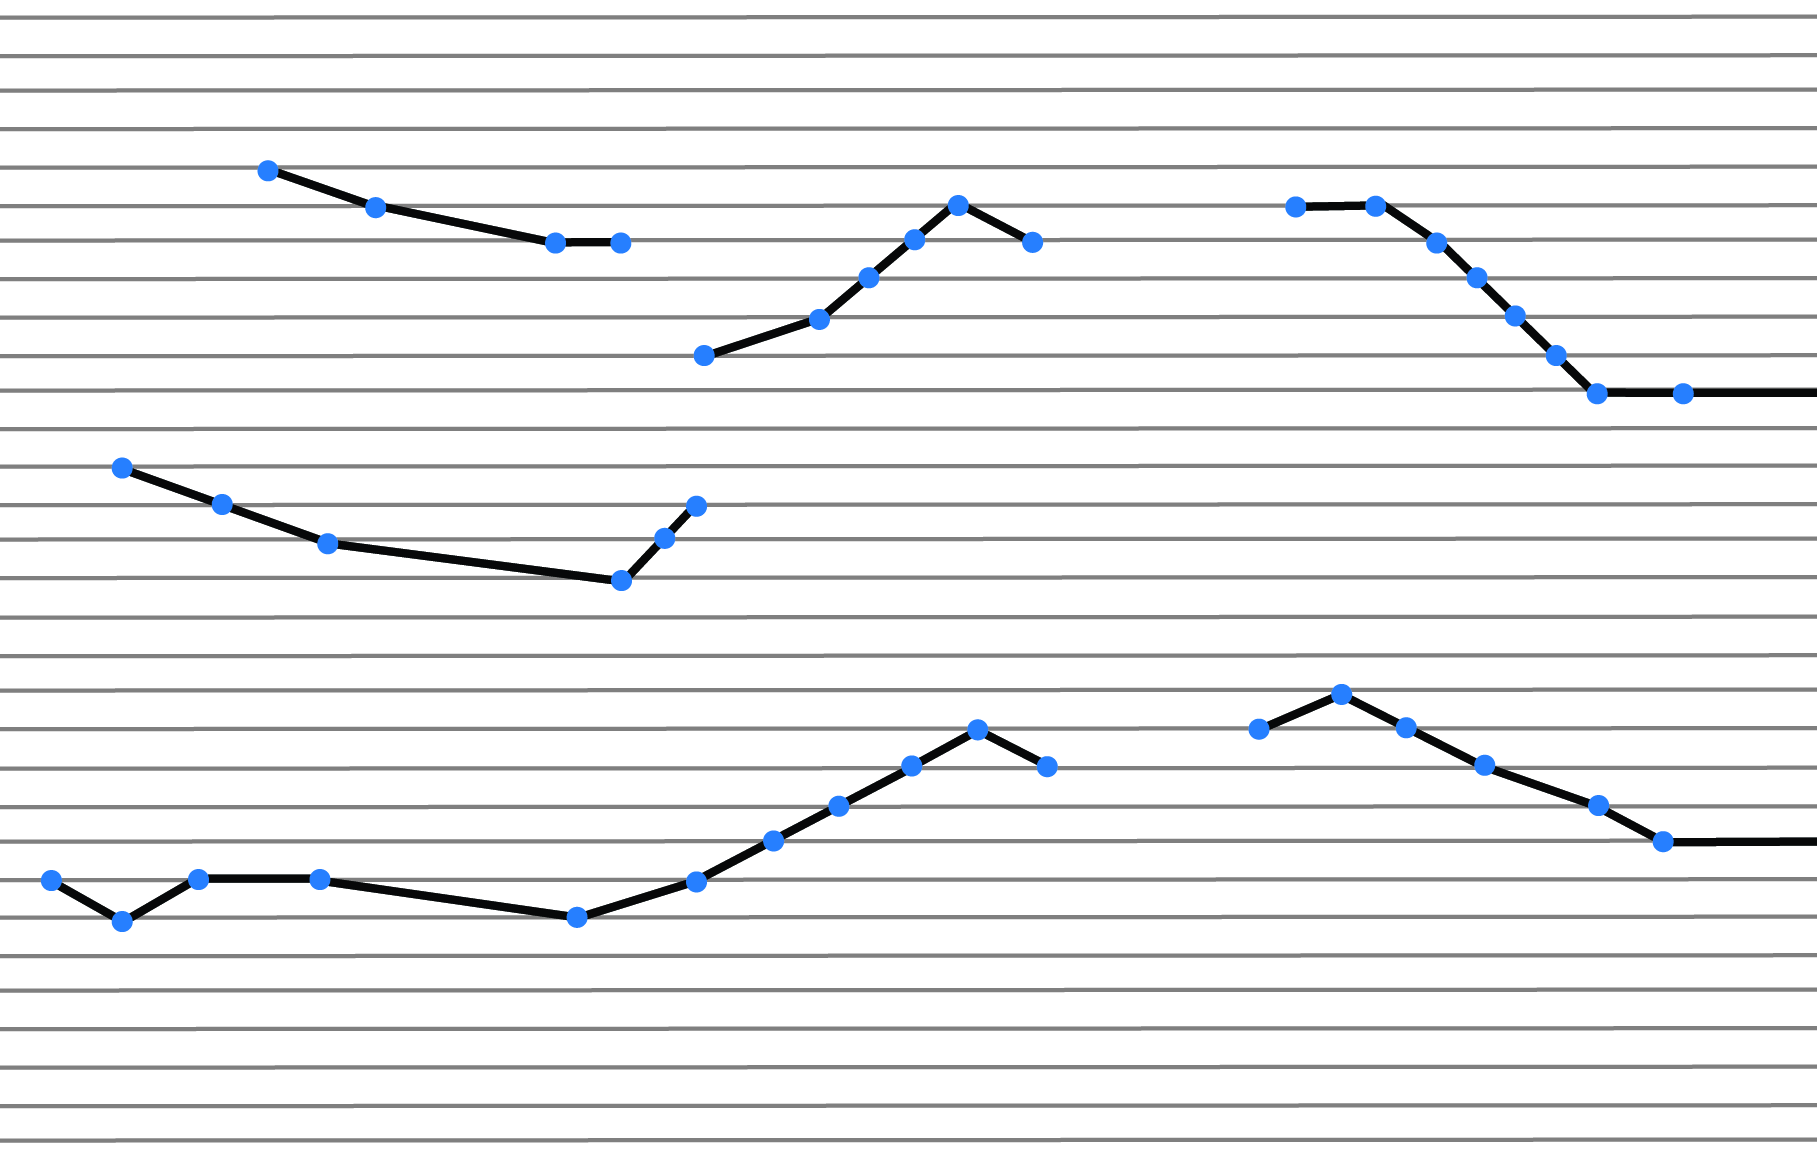
\includegraphics[width=10cm]{Chapter6/Spear3.tif} %change centimeters for resizeing
   \caption{SPEARToMIDI: Point selection through frequency modulation threshold.}
   \label{fig:example}
\end{figure}\
If the interval is of one semitone then the frequencies are averaged to the closest chromatic note. It is possible to make microtonal divisions of the equal-tempered scale by using floating point values for the modulation threshold. The magnitude, frequency and time values of each point are stored as a collection of data. This collection can then be accessed and used to control synthesis definitions externally by generating envelopes, which gradually change frequency to produce glissandos and amplitude for gradual volume change. After these first two stages, the original data from Spear is reduced considerably by disregarding details that are not vital for the given purpose. 

The third stage, takes the points of the lines that were obtained in the previous stage and translates them into single notes with a start and an end and that do not change in frequency and amplitude while playing--- in other words, a format that is compatible with the Midi note-on and note-off paradigm. The points are then considered as representing note-on messages and the note-off messages are calculated depending on whether the point is followed by another new point or if the point is the last of the group, in which case a silence would proceed. In other words, a note-off is inserted before a new note-on or just before a silence. Figure 4.7 
\begin{figure}[htbp] %  figure placement: here, top, bottom, or page
   \centering
   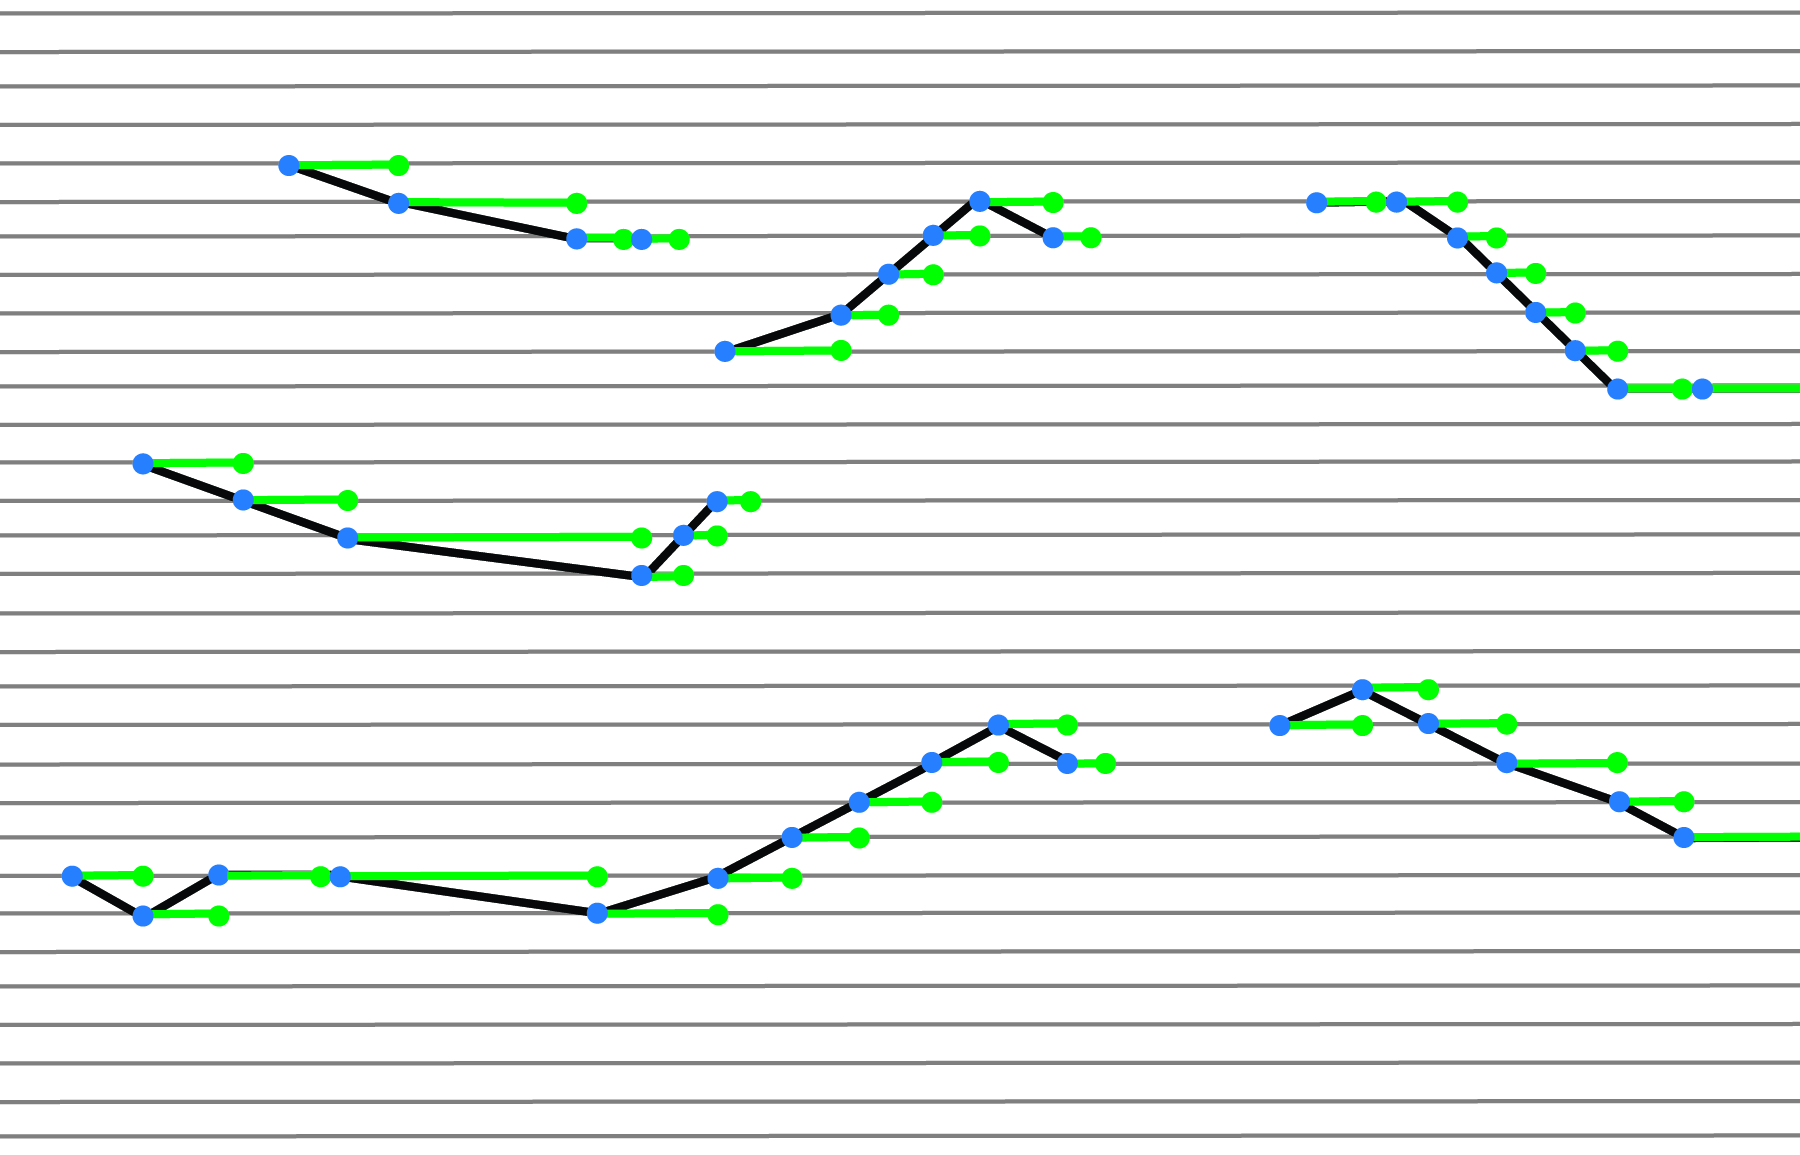
\includegraphics[width=10cm]{Chapter6/Spear4.tif} %change centimeters for resizeing
   \caption{SPEARToMIDI: Note representation.}
   \label{fig:example}
\end{figure}\
shows the note representation derived from Figure 4.5, where the notes are seen as green lines, the note-on messages as blue points and the note off messages as green points. 
The results of this stage can be used to generate a Midi file\hypertarget{wlib}{}\footnote{Using the SimpleMIDIFile class that is part of wslib by \href{http://www.woutersnoei.nl/}{Wouter Snoei}, which is can be obtained as a Quark.} with the intention of either using it to trigger a sampler or to import it into a notation software to create a written score. The user can input the time signature and tempo for the Midi file as well as an interval value that divides the Midi note range into different Midi tracks. By doing this, the notes are separated into different tracks depending on their value in relationship to each other with the purpose of not having too many notes in the same track. Furthermore, these results can be used to create a list of Open Sound Control (OSC)\footnote{See \href{http://opensoundcontrol.org/introduction-osc}{http://opensoundcontrol.org/introduction-osc}.} commands that can be sent to the SuperCollider server for Real-Time-Synthesis and Non-Real-Time-Synthesis. Extra arguments can also be added to control other values in the synthesis definition, which can be set individually by using a function to be evaluated for each instance of the definition.

\section{Computer-Mediated-Performance}

\subsection{Real-Time Scoring}

\emph{Interpassivity.} Improvisation, etc.
Display as score. Score animations...
Computer conductor.
Computer-aided conducting... Human decides in real-time sections, etc.

\subsubsection{AlgorithmicScore}

\href{http://github.com/freuben/FedeLib/blob/master/AlgorithmicScore/AlgorithmicScore.sc}{AlgorithmicScore} is a class that visualizes different types of notation in real-time. It is programmed as a graphical user interface (GUI) in SuperCollider but receives no input in the GUI window itself. Instead, this class only displays notes, letters, symbols and other visual aids for real-time scoring from code that can be evaluated in the interpreter, or within a compiled class in the SuperCollider language. It displays traditional musical symbols including notes, accidentals, clefs and dynamics that are available as fonts\footnote{The fonts I used for the AlgorithmicScore class are MusiSync by Robert Allgeyer and Sonora by Christian Texier.} in combination with non-standard notations. Stems and flags are purposely not implemented so that too much visual information is not given to the performer while following the score. Note-heads can be of different type and color. There are four types of different clefs that are implemented: treble, bass, alto, tenor.  If a clef is selected, a staff is generated in which the notes will appear. The information to be placed in the score can be evaluated in an array consisting of the note position from left to right, staff number, note-head type, note, accidental and color. There are three array types that can be used which respond to different notation modes: free, enharmonic and chromatic. In the free mode, notes are selected by a number that does not correspond to the clef but to the position from top to bottom starting with zero as the first leisure line bellow the bottom line of the staff. Moreover, the note value can not only be negative but also a float number, which results in a position in between notes. This mode can be useful for conveying movement if the score were to be animated. The enharmonic mode, takes a string representing the note and octave---were c4 equals middle C---and positions the note according to the selected clef. It is also possible to select the type of accidental between flat, sharp and natural. If the note exceeds four leisure lines, the programme places an \emph{8va} sign and if it is exceed it by yet another octave, it places a \emph{15ma} sign. The chromatic mode, is similar to the enharmonic, but only uses sharps as accidentals and places a natural in front of each note that is diatonic. This mode is useful to receive note information as Midi numbers. In addition, it is possible to place written directions with different colors in the score.

The following code example produces a score in real-time if evaluated from the interpreter window: 
\begin{verbatim}
a = AlgorithmicScore.screenBounds; //start class
a.score([\bass, \treble, \treble]); //3 staffs
//[pos, [staff, noteType, note, acc, color]]:
~staff1 = [[0, [0, 1, "c3"]], [1, [0, 0, "b3", \flat, \blue]]]; 
~staff2 = [[0, [1, 0, "d5", \flat]]];
~staff3 = [[0, [2, 1, "a3", \nat, \red]]];
a.enharmonic(~staff1 ++ ~staff2 ++ ~staff3); //writes notes
a.expression("p"); //expression for dynamics
a.text("Improvise with pitch material", "Helvetica", 30, 30, 200, color: Color.rand);
//string, fontType, letterSize, inLeft, inTop, color  
\end{verbatim}
The code generates a new window and three staffs with one bass and two treble clefs. The separate arrays correspond to each staff\footnote{Note that the first value is for the position of the note from left to right and that the values are already scaled so that in the entire length of screen can fit 24 notes.} and are concatenated to respond to the enharmonic mode. In addition, an expression to play \emph{piano} and a text description are added. Figure 4.7 shows the GUI that the AlgorithmicScore class creates when the code above is evaluated. 
\begin{figure}[htbp] %  figure placement: here, top, bottom, or page
   \centering
   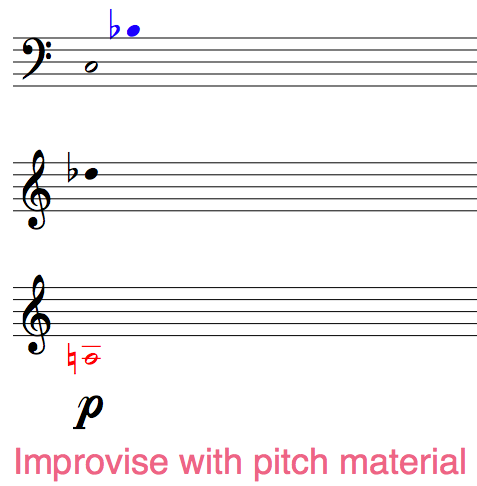
\includegraphics[width=9cm]{Chapter6/algoscore1.tif} %change centimeters for resizeing
   \caption{AlgorithmicScore: Enharmonic mode.}
   \label{fig:example}
\end{figure}\

Another feature of the application is a piano clef type which instead of creating only one staff that responds to the corresponding clef, it produces two staffs with one treble clef on the top staff and one bass clef on the bottom staff. In this clef type, the note is placed on the treble clef staff if it is higher or equal to middle C and if it is lower than middle C, it is placed on the bass clef staff. Furthermore, it is possible to score in real-time by evaluating an array of Midi note numbers. The class takes the Midi numbers and translates them to the correct pitch type and octave in the chromatic mode. This procedure is a very convenient form of sending Midi values to be scored in real time. The following example of code takes sixteen random notes from f1 to g6 and chooses one of them randomly and changes its color to red:
\begin{verbatim}
a = AlgorithmicScore.screenBounds; //start class
a.score([\piano]); //piano staff
~notes = Array.fill(16, {rrand("f1".notemidi,"g6".notemidi)}); 
//random notes between f1 and g6
~color = Array.fill(~notes.size, \black).insert(rrand(0,15),\red);
//all notes black, except a random red note
a.notes(~notes, color: ~color);
\end{verbatim}
\begin{figure}[htbp] %  figure placement: here, top, bottom, or page
   \centering
   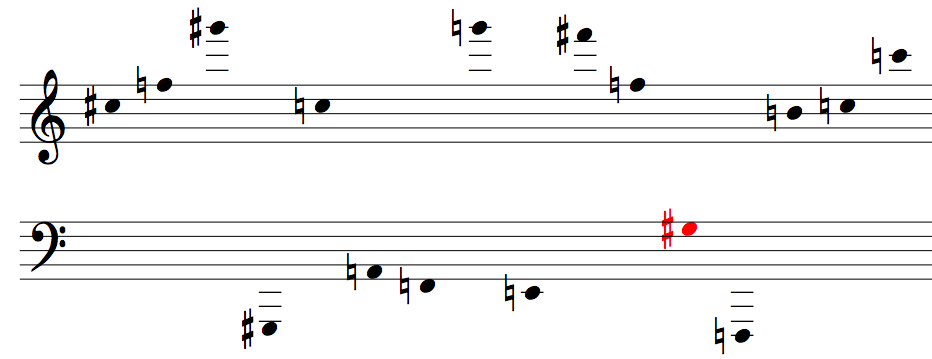
\includegraphics[width=14cm]{Chapter6/algoscore2.tif} %change centimeters for resizeing
   \caption{AlgorithmicScore: Chromatic mode.}
   \label{fig:example}
\end{figure}\
The \emph{notes} message\footnote{A message is the type of operation that the class performs depending on the type of message it receives.} takes as input one array of notes, one of positions and one of colors. If the array of positions is not specified, the computer arranges the positions equally from left to right. Figure 1.8 shows the resulting score generated by the code. Note that the notes are spread between the treble and bass clefs because the piano clef type is selected. 

This method for generating scores can be very useful to notate pre-composed and aleatoric material in real-time. Moreover, this application is ideal to to visualize pitch or rhythmic information derived from machine listening techniques such as partial tracking. Real-time scoring is specially relevant when using machine listening applications because the material that is notated is extracted from sound characteristics that are specific to the moment and space of the performance. \mbox{Figure 1.9} shows an example that uses the \hyperlink{partrack}{PartialTracker} class to extract Midi note numbers from the strongest twenty partials of a spectrum. The resulting score is therefore generated in real-time and is specific to the space and time in which the partials are extracted.
\begin{figure}[htbp] %  figure placement: here, top, bottom, or page
   \centering
   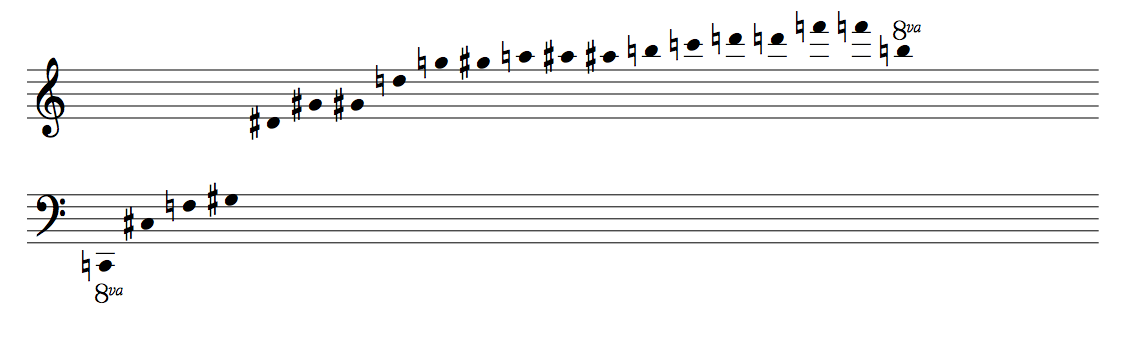
\includegraphics[width=17cm]{Chapter6/algoScore_partials.tif} %change centimeters for resizeing
   \caption{AlgorithmicScore: PartialTracker to Notes.}
   \label{fig:example}
\end{figure}\

A sense of movement can be generated using the AlgorithmicScore class if the notes and other graphics are imbedded within a \emph{routine}.\footnote{Routines in SuperCollider are functions used for scheduling timed events using a clock that can be specified.} Therefore, it is possible to animate the graphical user interface including the notation elements for different purposes. One purpose for using score animations is to convey a sense of gesture by animating the notes so that they appear to be moving in specific directions. It is possible then to make notes appear as if they are skipping or jumping by changing note values every time an element of the \emph{routine} is evaluated.\footnote{For example, see URL: \href{http://www.youtube.com/watch?v=QhJdffgLhZA}{http://www.youtube.com/watch?v=QhJdffgLhZA}.} It is also possible to achieve a sense of a note gradually moving horizontally by gradually changing the numbers for the position of a note. In addition, one can animate the direction vertically by gradually changing the note values in free mode.\footnote{See URL: \href{http://www.youtube.com/watch?v=m5GBfeUDeUA}{http://www.youtube.com/watch?v=m5GBfeUDeUA} for an example of notes gradually moving horizontally and vertically.} Furthermore, generating movement in real-time scoring can express timing and other conducting cues and gestures. The AlgorithmicScore class gives the possibility of scheduling a mixture of written directions, notation, chronometers, arrows and other graphics.  Visual cues can be given through the computer display to signal the beginning and end of sections as well as other important timing instructions. The use of colors to indicate silence and new sections is also possible when using this class.\footnote{See the \href{http://www.youtube.com/watch?v=m5GBfeUDeUA}{\emph{Zizek!?} Score} for an example of this application of real-time scoring.} 

Given that the AlgorithmicScore class does not use note stems and flags as an element of notation, rhythm may be expressed visually as well as aurally. Rhythm might be expressed with score movement using visual triggers that turn \emph{on} and \emph{off} symbolizing the onset and release of a note---this class has circular triggers that switch between bright colors (\emph{on}) and light grey (\emph{off}) to covey rhythm.\footnote{For example, see URL: \href{http://www.youtube.com/watch?v=Rw58E_y3GT4}{http://www.youtube.com/watch?v=Rw58E\_y3GT4}.} Another strategy to express rhythm through score movement is by changing the color of only one note at a time within a sequence of notes---the logical movement being from left to right.\footnote{For example, see URL: \href{http://www.youtube.com/watch?v=sCE6rLJgdwk}{http://www.youtube.com/watch?v=sCE6rLJgdwk}.} Aural triggers may be added to indicate both rhythm and pitch by producing sounds that will serve as guide to the performer. The sounds would account for an aural score that the performer would receive through headphones and might enhance the visual elements of the AlgorithmicScore class.

Additionally, it is possible to import any type of image and video within the class and therefore create a wide variety of non-standard graphical indications. This application also provides the option to import scores written traditionally in standard notation programmes and combine them with the more expressive potential of the AlgorithmicScore class. Finally, by using human interface devises (HIDs) such as Midi controllers and pedals the performer may interact with the score. This might be helpful for example to trigger score animations or turn pages with a Midi pedal. Other examples of human-to-score interaction include controlling tempo and conducting cues with human gesture and triggering spectral data extraction to be displayed in the computer display with different types of sensors. 

\section{Computer-Aided-Composition Tools}

As part of my creative output, I have developed computer applications that served me as computer-aided-composition (CAC) tools during my research. This set of tools can be found in a library of  SuperCollider classes and extensions called \href{http://github.com/freuben/FedeLib}{FedeLib}. An important component to this library is a collection of extensions\footnote{These extensions can be found at URL: \href{http://github.com/freuben/FedeLib/tree/master/Extensions/}{http://github.com/freuben/FedeLib/tree/master/Extensions/}.} to existing classes that perform a wide variety of tasks. These tasks include: mathematical operations on simple numbers and lists; musical calculations including different types of tuning systems, interval and pitch-class recognition, scale generation and voice leading; scheduling and time related applications; operations on strings; envelope generation; recurrent operations such as recording audio, handling Midi, switching between servers, managing buffers and patterns; Midi file analysis, transformation and triggering; and GUI creation. These tools aided me in the composition of the works submitted and might be useful to other composers. They too might reflect some of my compositional interests and methods. Nevertheless, I will not attempt to describe all extensions as it would be out of the scope of this discussion. Therefore, I will focus only on a few tools that I think are fundamental in my creative process as they are related with the concepts described in the previous chapters.

\subsection{Score Visualization}

During several years, I have developed pre-compositional tools that help me organize my music and think in terms of structure at different levels of abstraction. I normally start a piece of music with an idea of a macro-structure and then gradually start considering the micro-elements of the composition. That is to say, usually I first establish a foundation or blueprint that determines the structural decisions of a composition before I start working on the details that are related to smaller temporal intervals. As I became interested in deriving elements of existing compositions in my work, I decided to abstract other pieces of music by other composers that I consider excel in dealing with macro-structure. Therefore, I started by analyzing the score of these compositions and then tracing their phrase structure that I would use as a blueprint for my own composition. Each voice or staff would be considered as different layers containing phrases that would start and end depending on where silences occur. I would then create `empty containers' with the phrase structure of each voice of the appropriated composition. Consequently, I would sketch in a piece of squared paper the start and end of phrases according to a time scale. Ones I would sketch a diagram of ``empty containers'', I would start thinking what sonic `material' I would fill the containers with and how this `material' would develop. Normally, I would also treat this `material' by processing it with information derived from the melodic contour of the original phrases and relating it to the harmonic elements of the original composition. As I become more experienced as a composer, I adhere less to this idea of thinking of music as controlled layers of sound or music and take less rigid interpretation of these blueprints. Nevertheless, I still always begin by reducing an existing score by another composer to its basic marco-elements as a starting point for my own composition. 

Considering that this is a process that is recurrent in my compositional practice and I always sketch the phrase structure of the existing scores similarly on paper, I decided to programme an application in SuperCollider that takes information from a Midi file and creates a visualization of its phrase structure. Therefore, I developed extensions for the SimpleMIDIFile\footnote{SimpleMIDIFile accesses Midi file information in SuperCollider. See footnote number \hyperlink{wlib}{14}.} class to perform these operations. The message \emph{trackSilence}\footnote{See URL: \href{http://github.com/freuben/FedeLib/blob/master/Extensions/FedeExtensions.sc}{http://github.com/freuben/FedeLib/blob/master/Extensions/FedeExtensions.sc} for the FedeLib extensions including SimpleMIDIFile's \emph{trackSilence} message.} analyses a Midi file\footnote{The Midi file's content must have the standard Midi layout and specifications for scored music. If a Midi file does not follow this specifications, it can be edited so that it meets the requirements for a coherent visualization.} track and locates the starting and ending points of silences. The application analyses the Midi note-on and note-off messages and finds the moments where notes are not being played. It is possible to specify a time threshold (either in ticks or seconds) that ignores silences smaller than the given value. This way silences that are shorter than those which are notated may be ignored such that only the written silences are considered. The following example shows  the results given in a multidimensional array that specifies the start and end times of the silences.
\begin{verbatim}
[ [ 17.14284, 17.92206 ], [ 38.961, 40.51944 ], [ 50.416336, 51.034892 ], 
[ 56.601896, 57.220452 ], [ 70.210128, 72.065796 ], [ 88.77462, 89.154366 ], 
[ 95.610048, 96.36954 ], [ 105.483444, 106.242936 ], [ 118.394808, 119.1543 ] ]
\end{verbatim}

Ones the results for the timings of silences for each track of the Midi file are obtained, it is possible to create a visualization of the phrase structures. The \emph{phraseStructure} message creates a GUI window that displays this information by converting time values to pixels to create a visual representation of the Midi file. Figure 4.10 shows the result of the visualization of a Midi file of a section of Johannes Ockeghem's \emph{Missa Mi mi}. 
\begin{figure}[htbp] %  figure placement: here, top, bottom, or page
   \centering
   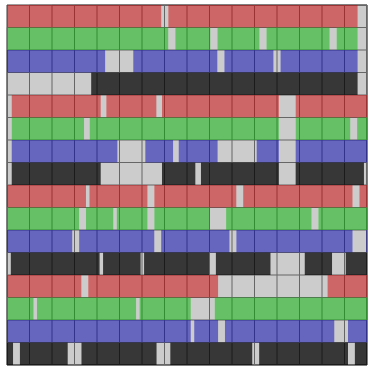
\includegraphics[width=8cm]{Chapter6/midi_phrase.tif} %change centimeters for resizeing
   \caption{Visualization of Ockeghem's \emph{Missa Mi mi}.}
   \label{fig:example}
\end{figure}\
Each Midi track is represented as a different color and the silences are displayed in light grey. The Midi tracks represent the different voices of the \emph{Missa Mi mi}, where the red stands for the \emph{discantus}, the green for the \emph{contratenor}, the blue for the \emph{tenor} and the black for the \emph{bassus}. The x-axis represents time and each square equals to a value for time that can be specified by the user. This enables the user to `zoom' in and out of the phrase structure. The combinations of this elements of representation result in a visualization of the phrase structure for each voice of the existing composition that may serve as a map of the structure or blueprint for the new work. The application can also produce a black and white printable version of the visualization. Figure 1.11 shows a printable version of the visualization of the Midi file of Gesualdo's madrigal \emph{Se la mia morte brami}. 
\begin{figure}[htbp] %  figure placement: here, top, bottom, or page
   \centering
   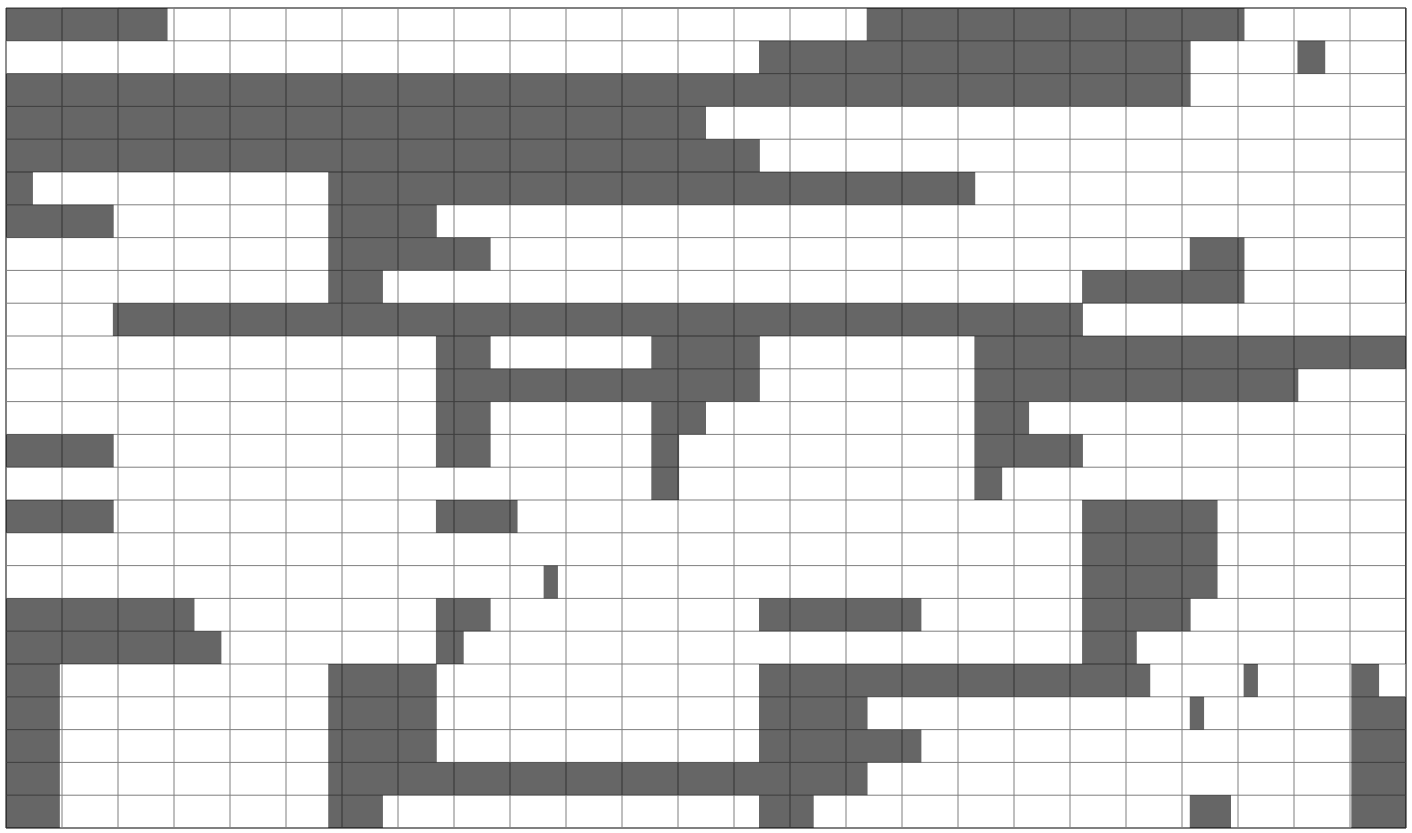
\includegraphics[width=16cm]{Chapter6/midi_gesualdo.tif} %change centimeters for resizeing
   \caption{Visualization of Gesualdo's \emph{Se la mia morte brami}.}
   \label{fig:example}
\end{figure}\
This Midi file has five tracks which represent the different voices of the madrigal. The representation of the Midi file displays the silences in dark grey and the phrases in white. This is with the purpose of being able to consider the phrases as `empty containers' and write annotations in the printed result on what kind of `material' these containers may be filled with. That is to say, the result can be used as a sort of pre-compositional design for the new composition and the printed version allows the composer to make notes on different levels of decision making through time.


\subsection{Midi Triggering}

Following the idea of using existing compositions as a blueprint for the design of a new work, I have continued to write applications that trigger events and processes through Midi messages. For example, these events or processes might be used to trigger and control synthesis definitions, Midi events and even real-time scoring. I have written various extensions of SimpleMIDIFile to use the messages from a Midi file for this objective. Therefore, these extensions employ a Midi file as a control structure for triggering functions of different types.
The extension \emph{playTrackType} plays different types of Midi events in a Routine. One can specify a track number, type of Midi event, function to be evaluated when the event is triggered, starting time for the Midi file and  value to change the tempo by multiplying it to the original tempo of the Midi file. The function that is evaluated contains as arguments the specifications of the Midi events---for example, Midi channel, note and velocity, which can be accessed by the user. Therefore, it is possible to use this values to control the events or processes of the new composition. Additionally, the \emph{sectionPlay} message uses the information obtained by \emph{trackSilence} to evaluate a function each time that a phrase or silence starts. Furthermore, the \emph{phrasePlay} message evaluates two different functions: the first is evaluated at the beginning of a phrase and the second at the beginning of a silence. This two extensions respond to the same arguments as \emph{playTrackType} and can be useful for controlling meta-structures. They can also be used by the AlgorithicScore class to give cues to performers or trigger score animations. 

Given that Midi files which are created with the information from a score are quantized and therefore can be lacking in expression for a given purpose, I have also designed similar applications that work with incoming Midi data from a human performer. Therefore, the computer can analyze the information in real-time and trigger events and processes that the composer programs before the performance. This type of application can be used in \emph{Real-Time Plunderphonics}\footnote{See pp  for an explanation of  the term.} as a strategy to control structures in a live performance.

\section{Live-electronics}

\subsection{Spectrum Driven Sampler}

\subsection{Improvisation Environment}

\label{ch:compapp}